\section{mo\-Gen\-Sol\-Continue$<$ EOT $>$ Class Template Reference}
\label{classmo_gen_sol_continue}\index{moGenSolContinue@{moGenSolContinue}}
One possible stop criterion for a solution-based heuristic.  


{\tt \#include $<$mo\-Gen\-Sol\-Continue.h$>$}

Inheritance diagram for mo\-Gen\-Sol\-Continue$<$ EOT $>$::\begin{figure}[H]
\begin{center}
\leavevmode
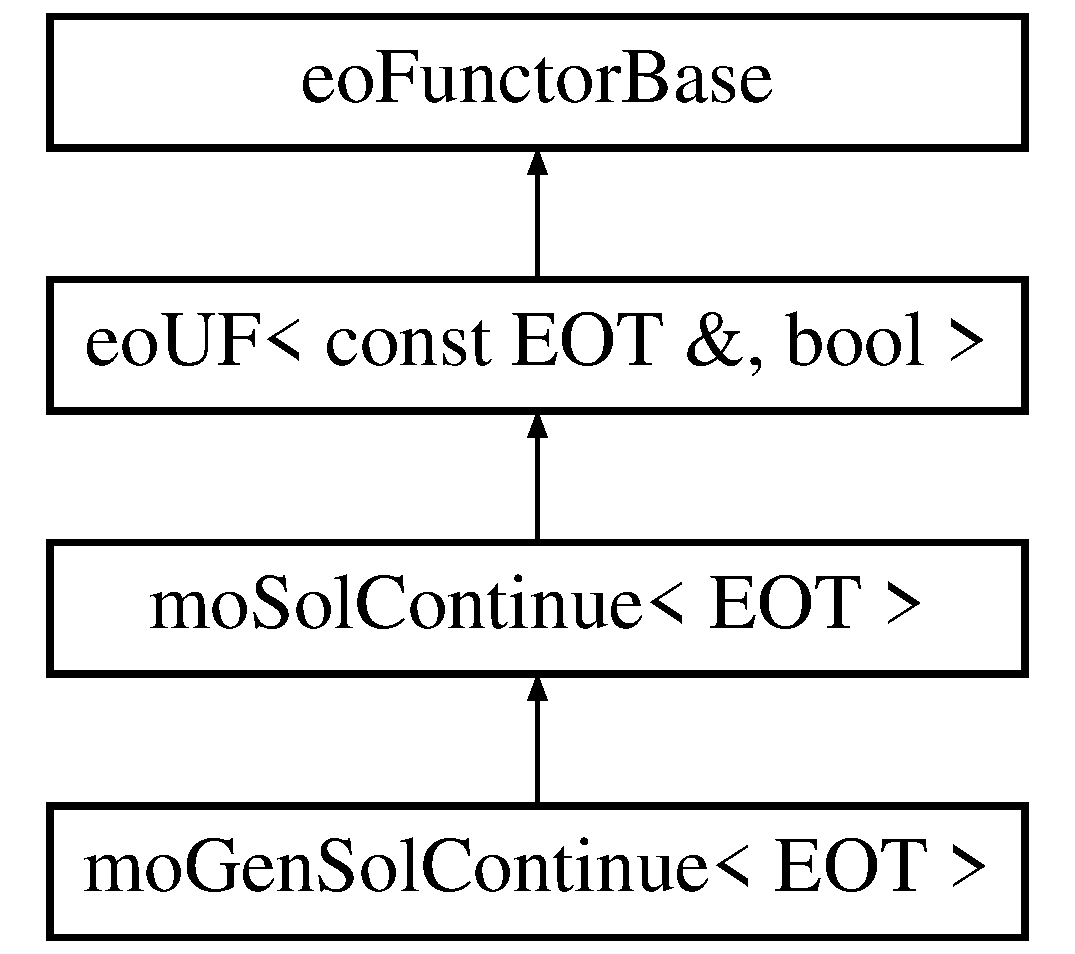
\includegraphics[height=2cm]{classmo_gen_sol_continue}
\end{center}
\end{figure}
\subsection*{Public Member Functions}
\begin{CompactItemize}
\item 
{\bf mo\-Gen\-Sol\-Continue} (unsigned \_\-\_\-max\-Num\-Gen)
\begin{CompactList}\small\item\em Simple constructor. \item\end{CompactList}\item 
bool {\bf operator()} (const EOT \&\_\-\_\-sol)
\begin{CompactList}\small\item\em Function that activates the stop criterion. \item\end{CompactList}\item 
void {\bf init} ()
\begin{CompactList}\small\item\em Procedure which allows to initialise the generation counter. \item\end{CompactList}\end{CompactItemize}
\subsection*{Private Attributes}
\begin{CompactItemize}
\item 
unsigned {\bf max\-Num\-Gen}\label{classmo_gen_sol_continue_6d7674fc51d17423e8ee28693a08b5af}

\begin{CompactList}\small\item\em Iteration maximum number. \item\end{CompactList}\item 
unsigned {\bf num\-Gen}\label{classmo_gen_sol_continue_a18ebfd270f96517b4edaa2cad3eb9e0}

\begin{CompactList}\small\item\em Iteration current number. \item\end{CompactList}\end{CompactItemize}


\subsection{Detailed Description}
\subsubsection*{template$<$class EOT$>$ class mo\-Gen\-Sol\-Continue$<$ EOT $>$}

One possible stop criterion for a solution-based heuristic. 

The stop criterion corresponds to a maximum number of iteration. 



Definition at line 21 of file mo\-Gen\-Sol\-Continue.h.

\subsection{Constructor \& Destructor Documentation}
\index{moGenSolContinue@{mo\-Gen\-Sol\-Continue}!moGenSolContinue@{moGenSolContinue}}
\index{moGenSolContinue@{moGenSolContinue}!moGenSolContinue@{mo\-Gen\-Sol\-Continue}}
\subsubsection{\setlength{\rightskip}{0pt plus 5cm}template$<$class EOT$>$ {\bf mo\-Gen\-Sol\-Continue}$<$ EOT $>$::{\bf mo\-Gen\-Sol\-Continue} (unsigned {\em \_\-\_\-max\-Num\-Gen})\hspace{0.3cm}{\tt  [inline]}}\label{classmo_gen_sol_continue_6b6cab23a23bd8904ea52ef5141d8d0a}


Simple constructor. 

\begin{Desc}
\item[Parameters:]
\begin{description}
\item[{\em \_\-\_\-max\-Num\-Gen}]the maximum number of generation. \end{description}
\end{Desc}


Definition at line 30 of file mo\-Gen\-Sol\-Continue.h.

\subsection{Member Function Documentation}
\index{moGenSolContinue@{mo\-Gen\-Sol\-Continue}!operator()@{operator()}}
\index{operator()@{operator()}!moGenSolContinue@{mo\-Gen\-Sol\-Continue}}
\subsubsection{\setlength{\rightskip}{0pt plus 5cm}template$<$class EOT$>$ bool {\bf mo\-Gen\-Sol\-Continue}$<$ EOT $>$::operator() (const EOT \& {\em \_\-\_\-sol})\hspace{0.3cm}{\tt  [inline]}}\label{classmo_gen_sol_continue_457257cd73b474d6f7783d84d02c2e61}


Function that activates the stop criterion. 

Increments the counter and returns TRUE if the current number of iteration is lower than the given maximum number of iterations.

\begin{Desc}
\item[Parameters:]
\begin{description}
\item[{\em \_\-\_\-sol}]the current solution. \end{description}
\end{Desc}
\begin{Desc}
\item[Returns:]TRUE or FALSE according to the current generation number. \end{Desc}


Definition at line 44 of file mo\-Gen\-Sol\-Continue.h.

References mo\-Gen\-Sol\-Continue$<$ EOT $>$::max\-Num\-Gen, and mo\-Gen\-Sol\-Continue$<$ EOT $>$::num\-Gen.\index{moGenSolContinue@{mo\-Gen\-Sol\-Continue}!init@{init}}
\index{init@{init}!moGenSolContinue@{mo\-Gen\-Sol\-Continue}}
\subsubsection{\setlength{\rightskip}{0pt plus 5cm}template$<$class EOT$>$ void {\bf mo\-Gen\-Sol\-Continue}$<$ EOT $>$::init ()\hspace{0.3cm}{\tt  [inline, virtual]}}\label{classmo_gen_sol_continue_6c5db8182157584b56507cc9075602d4}


Procedure which allows to initialise the generation counter. 

It can also be used to reset the iteration counter. 

Implements {\bf mo\-Sol\-Continue$<$ EOT $>$} {\rm (p.\,\pageref{classmo_sol_continue_064dc966a210f4ffb9515be3f03ca4c7})}.

Definition at line 54 of file mo\-Gen\-Sol\-Continue.h.

References mo\-Gen\-Sol\-Continue$<$ EOT $>$::num\-Gen.

The documentation for this class was generated from the following file:\begin{CompactItemize}
\item 
mo\-Gen\-Sol\-Continue.h\end{CompactItemize}
